\documentclass[12pt]{report}
\usepackage[english]{babel}
\usepackage[utf8x]{inputenc}
\usepackage{amsmath}
\usepackage{graphicx}
\usepackage[colorinlistoftodos]{todonotes}
\usepackage{graphicx}
\usepackage{float}
\usepackage{subfigure}
\usepackage{algorithmic}
\usepackage{algorithm}
\usepackage{pdfpages}
\usepackage{color}
\usepackage[toc,page]{appendix}

% % % % % % % % % % % % % % % % % % % % % %
\begin{document}
% % % % % %Front Page % % % % % % % % % % %
\begin{titlepage}
\center

\textsc{\large Seminar Report On}\\[1.0cm] % Name of your university/college
\textsc{\Large BLOCKCHAIN IN HEALTHCARE DOMAIN}\\[1.0cm] % Major heading such as course name
\textsc{\large Submitted in Partial Fulfillment of the Requirements for the award of \\ Bachelor of Technology in \\ Computer Science and Engineering\\ (2015-2019)}\\[0.5cm] 

\begin{figure}[H]
\centering

\includegraphics[width=0.7\textwidth]{logo.png}\\
%\label{logo}
\end{figure}

\vspace{2.0cm}

\begin{minipage}{0.4\textwidth}
\begin{flushleft} \large
\emph{Submitted By:}\\
\hspace{0.3cm}Basil K Y\\
\hspace{0.3cm}Reg No. 15CS087\\
\end{flushleft}
\end{minipage}
~~~~~~~~~~~~~~~~~~~~
\begin{minipage}{0.4\textwidth}
\large
\emph{Guide:} \\
\color{white}...\color{black}Mr. Bineeth Kuriakose\\
\color{white}...\color{black}Department of CSE 
\end{minipage}\\[2cm]

\textbf{Department of Computer Science and Engineering}\\
\textbf{Muthoot Institute of Technology and Science (MITS)} \\
Varikoli P.O, Puthencruz-682308
\end{titlepage}
% % % % % % % % % % % % % % % % % % % % % % % % %
\newpage\begin{titlepage}
\center


\textsc{ \textbf{MUTHOOT INSTITUTE OF TECHNOLOGY \& SCIENCE}}\\
\textsc{\textbf{Varikoli P.O, Puthencruz-682308}}
\vspace{0.7cm}
\begin{figure}[H]
\centering

\includegraphics[width=0.7\textwidth]{logo.png}\\
%\label{logo}
\end{figure}
\vspace{0.2cm}
\textsc{ \small \textbf{ DEPARTMENT OF COMPUTER SCIENCE \& ENGINEERING}}\\
\section*{\centering CERTIFICATE}
%\thispagestyle{empty}
\begin{center}
 This is to certify that the seminar report entitled "AYUSH : BLOCKCHAIN BASED HEALTH RECORD MANAGEMENT SYSTEM" submitted by \textbf{Basil K Y(15CS087)} of Semester VII is  a bonafide account of the work done by him/her under our supervision\\
\end{center}
\vspace{1.6cm}




\noindent Guide \hspace{3.6cm} Coordinator\hfill Head of the Department
\\
\noindent Mr. Bineeth Kuriakose\hspace{0.82cm}Ms Rakhee M \hfill Dr. Anand Hareendran\\
\noindent Asst. Professor\hspace{2.05cm} Asst. Professor\hfill Asso. Professor\\
\noindent Dept. of CSE\hspace{2.3cm} Dept. of CSE\hfill Dept. of CSE
%\noindent\textbox{Left longer sample text\hfill}\textbox{\hfil Center\hfil}\textbox{\hfill Right




\end{titlepage}
\newpage
\pagenumbering{roman}

\section*{\centering Acknowledgements}
\par This seminar is the result of my hard work wherein I have been helped and supported by several persons and institutions directly and indirectly. Now it is the time to acknowledge their contributions. 

\par First of all to the Great Almighty, the author of knowledge and wisdom for his countless love. I respect and thank \textbf{Dr.Chikku Abraham}, Vice Principal of MITS for giving me the opportunity to do this seminar.
With great respect, I express my sincere thanks to our Head of The Department \textbf{Dr. Anand Hareendran} for all the proper guidance and encouragement. I extent my gratitude to the seminar coordinators \textbf{Asst. Prof.Rakhee M}, \textbf{Prof. Dr. Raju.C.K} and \textbf{Asst. Prof. Resmi.N.G} for their timely advice, meticulous scrutiny, scholarly advice and scientific approach that helped to a very great extent throughout the seminar. I would like to sincerely thank my guide \textbf{Asst. Prof. Bineeth Kuriakose}, for her support and valuable guidance.

\par I express my heartfelt veneration to all who had been helpful and inspiring throughout this endeavour.


\null\hfill Basil K Y
\newpage

\section*{\centering Abstract}
Blockchain is an emerging technology with tremendous applications in various sectors including healthcare.A number of blockchain based solutions and concepts have been emerged to solve or to find enhanced solutions for existing problems in healthcare sector.Many multinational companies are also confident in investing on blockchain over healthcare.The decentralized peer to peer networking of blockchain can ensure trust between participants in the network.Even though technology behind is blockchain, there are differences in implementation concepts.
In this seminar I will be listing major problems in healthcare, together with potential solutions using blockchain technology.
\newpage



\tableofcontents
\addcontentsline{toc}{chapter}{List of Figures}

\listoffigures
%\addcontentsline{toc}{chapter}{List of Tables}
%\listoftables

% % % % % % % %% % % % % % % % % % % % % % % % % %

\chapter{Introduction}

Blockchain is a distributed and decentralized chain of records or ledgers.The immutability of blockchain records ensures trust between participating entities.At its core, blockchain is a distributed
system for recording and storing transaction
records. More specifically, blockchain is a
shared, immutable record of peer-to-peer
transactions built from linked transaction
blocks and stored in a digital ledger.
Blockchain relies on established
cryptographic techniques to allow each
participant in a network to interact (e.g.
store, exchange, and view information),
without preexisting trust between the
parties. In a blockchain system, there is no
central authority; instead, transaction
records are stored and distributed across all
network participants. Interactions with the
blockchain become known to all participants
and require verification by the network
before information is added, enabling
trustless collaboration between network
participants while recording an immutable
audit trail of all interactions.This has lead to a wide range of applications for blockchain on different domains like banking,financial transactions,social media platforms,crypto currencies etc.The impact of blockchain technology can also be seen in the healthcare industry also. Technologists and healthcare providers and professionals across the globe view blockchain technology as a crucial way to implement the sharing of medical records in a secure way to protect patient's personal data from outsiders, and give patients more control over their information.Various blockchain based solutions have been emerged to enhance current situation of healthcare.
\pagenumbering{arabic}

\chapter{Problems in Healthcare Sector}

The current healthcare infrastructure has often been called inadequate to handle information exchange and requires certain tweaks.Health record sharing in current scenario doesn't take care about the privacy of patients and patients have less control over their own data.The following is a list of main problems healthcare industry and the patients faces today.
\section{Interoperability of healthcare data}
Currently, there is no accepted standard for the sharing of health data from one hospital to another.Most of the cases, patient has to carry all of his past medical records to the new hospital or have to do the previous medical tests again.It’s difficult to simply copy information from one piece of EHR software to another. Mismatched types, strange data fields, and proprietary formats mean that data has to be manipulated and sanitized before it can be imported into another system. This lack of a common standard for capturing, transmitting, receiving, storing, and managing patient data causes delays and inaccuracies.Some EHR and healthcare system vendors are holding patient data for ransom. They charge fees for transmitting data outside the system, increasing operational costs and making providers less likely to send data to others in the healthcare supply chain. The government is acting to encourage interoperability, but not all vendors have taken this on board.There is no way to consistently identify a patient across multiple systems or providers. Patients can give their name, date of birth, and other identifying data, but because different systems store this information in different ways, errors are possible. There is a push towards a unique patient identifier — a code that could be used to categorically identify the same individual no matter what system or provider they used. Unfortunately, we are still far from getting this most basic of functionalities in place.There is also a lack of standards for sending, receiving, and managing information between EHR systems.
%1. What have you learned from the existing solutions\\
%2. What were the key points in selecting your work\\
%3. What were the drawbacks you spotted in the existing literature\\
\section{Fragmented patient records}
Patient data is scattered across many hospitals and healthcare service  providers. Patient doesn't have a longitudinal list of his/her past health records.Duplication of health records can occur within hospitals also.Different records may be generated for same patient if he forgets his unique IDs.Many hospitals in rural areas are still following physical records which makes the record handling even complex.The records are more prone to tampering and loss.
Patients regularly encounter fragmented systems of care and the results often lead to unmet social needs, conflicting medications, incorrect dosages etc. Many of patients that are the most affected by fragmented care coordination are populations that are already at-risk for chronic illnesses and have an array of unmet social needs. 
\section{Claim Adjudication}
Current existing patient billing management systems are at best complex and prone to manipulation by the
service providers – today, an estimated 50\% of healthcare costs are fraudulent, resulting from excessive
billing or billing for non-performed services.Also Currently, 20\%[bookchapetr2018] of claims get rejected either because they are not received by the insurer or they contain defects, such as incomplete or incorrect demographic
data or lack of proof supporting the services billed.There is a lack of trust between participants in the healthcare industry as medical records are easily changed by hospitals or patients for getting health insurances.It is easy to tamper the data if it is stored centrally at a place.Currently, twenty-two percent of claims get rejected either because they are not re-
ceived by the insurer or they contain defects, such as incomplete or incorrect demographic
data or lack of proof supporting the services billed.So,it is important to ensure that all
claims submitted for payment are coded accurately.
\section{Data Privacy and Security}
Since patient doesn't has the full control over his data, third parties can easily misuse the data.There are currently no mechanism available to share data in a permissioned and time bound manner.Sensitive data in healthcare can include patient data like protected health information (PHI), stored data such as medical and payment records, medical devices data etc. which are ubiquitous in healthcare environments.But healthcare organizations are not always properly prepared for managing and protecting their big data. That’s because IT departments within healthcare organizations often lack the budget necessary to bolster big data security.Data breaches, like the one that exposed nearly 38 million Anthem Health Insurance patient records, are becoming increasingly common. The healthcare industry has the highest risk factor when it comes to experiencing a data breach. Statistics show 88\% of all ransomware attacks in 2017 targeted the healthcare industry.[https://www.zettaset.com/index.php/solutions/data-privacy-protection-healthcare/].Healthcare records are considered highly valuable to cyber-attackers. This is because of the richness of personal, medical, financial information contained within each EHR. Data thieves can easily resell this information on the dark web. With access to this information, identity theft, insurance fraud, and financial fraud is committed for financial gain by criminal elements.But data is at risk even if an organization does not suffer an outside attack. Information can be leaked internally when employees, contractors, and IT security personnel do not take the proper precautions to manage and protect their data.
\section{Data Reliability}
Health data of patients should be instantly accessible when there is a need.Most of the service providers are storing health data locally in their database.This causes high potential for data reliability and data loss.If the system fails, entire patient health records gets destroyed.Cloud based duplication of data is necessary to reliably store data loss.


\chapter{Blockchain Applications in Healthcare}
\section{Personal Health Records}
\subsection{Medrec}
As the name indicates,the blockchain is made in a chain like fashion in wgich each record is linked with previous one.This property of blockchain can be used to links health records of patient and hospitals.PHRs enable patients to control how their health information is used and shared, verify
the accuracy of their health records, and correct potential errors in the data.
\begin{figure}[H]
\centering
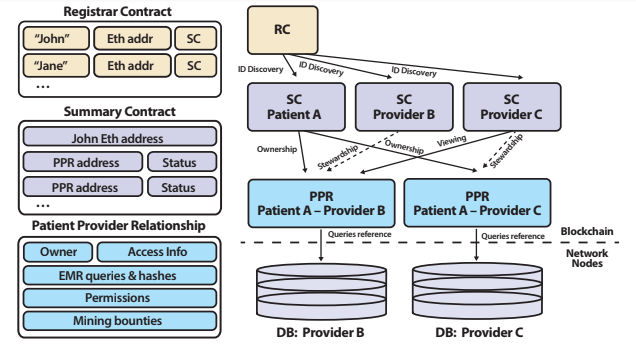
\includegraphics[width=0.7\textwidth]{ppr.png}
\caption{Personal Health Records}
\label{ppr}
\end{figure}
\subsection{Deloitte}
\section{Patient Controlled Data Sharing}
Consortium blockchain can be used to set access control to patient data.The access to the data can be made time based so that access to the patient data can be revoked after need or when patient want to block access.
\begin{figure}[H]
\centering
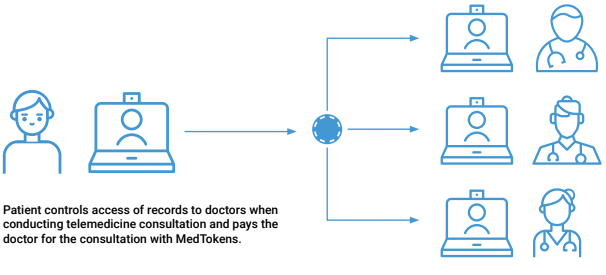
\includegraphics[width=0.9\textwidth]{sharing.png}
\caption{Patient Controlled Data Sharing}
\label{sharing}
\end{figure}
\section{Claim adjudication using smart contracts}
Smart contracts present
an opportunity for automating the adjudication process further by distributing and thus mak-
ing claims transparent to the provider and insurer, exposing potential errors and frauds that
can be corrected or investigated in a much timelier manner

\section{Ensuring trust between providers}
Blockchain's transparent behaviour can ensure trust between parcipating agents.Instead of creating a new trusted “middle man” that mediates the establishment of
trust relationships between providers/hospitals, Blockchain technology offers the opportunity
for trustless exchange and disintermediation that allow existing trust relationships to be ag-
gregated and propagated across various organizations and providers.

\section{Data Reliability}
Under blockchain, data is stored in a replicated manner and each participating node has complete copy of all the transactions.This replicated storage mechanism ensures reliability for stored data.

\chapter{Challenges in Implementation}
Even though there are good reasons behind applying blockchain on healthcare sector,as of now, there are no well established EHR management platform based on blockchain which actually works.There are services under development including Medicalchain,Medrec etc.Big multinational companies like IBM are also investing in blockchain.
\chapter{Conclusion}
\addcontentsline{toc}{chapter}{Bibliography}

\begin{thebibliography}{100} 

\bibitem{1} RJ Krawiec, Dan Housman, Mark White, Mariya Filipova,
Florian Quarre, Dan Barr, Allen Nesbitt, Kate Fedosova,
Jason Killmeyer, Adam Israel, Lindsay Tsai, \textquotedblleft Blockchain:
Opportunities for Health Care\textquotedblright, \textit{Department of Health and Human Services’ Office of the National Coordinator for Health
Information Technology (ONC) ideation challenge—The Use of Blockchain in Health IT and Health-Related Research}, August,2016.


\bibitem{2} Ariel Ekblaw, Asaph Azaria , John D. Halamka, MD, Andrew Lippman, \textquotedblleft A Case Study for Blockchain in Healthcare:
“MedRec” prototype for electronic health records and medical research data\textquotedblright, \textit{MIT Media Lab,Beth Israel Deaconess Medical Center}, August,2016.


\bibitem{3} \textquotedblleft Blockchain: The Chain of Trust and its Potential to Transform Healthcare – Our Point of View\textquotedblright, \textit{IBM Global Business Services Public Sector Team 6710 Rockledge Dr., Bethesda, MD 20817}August 8, 2016.

\bibitem{4} Richa Sharma, \textquotedblleft BLOCKCHAIN: the magic pill to alleviate the pain
points of the healthcare industry?\textquotedblright, \textit{France Canada Chamber of Commerce Ontario},June 5, 2018.

\bibitem{5}Kefa Rabah Mara Research, Nairobi Kenya,\textquotedblleft Challenges and Opportunities for Blockchain Powered Healthcare Systems: A Review\textquotedblright, \textit{Mara Research Journal of Medicine and Health Sciences} October 2017.

\bibitem{6}U. Krieger,T. Mundie,W. Liu,\textquotedblleft Advanced Block-Chain Architecture for e-Health Systems\textquotedblright, \textit{IEEE International
Workshop on Emerging Technologies for Pervasive Healthcare and Applications} 2017.


\bibitem{7} \textquotedblleft Applications of Blockchain Within Healthcare\textquotedblright[Online]\\ 
\textit{Available: https://doi.org/10.30953/bhty.v1.8}


\bibitem{8} \textquotedblleft Medicalchain\textquotedblright[Online]\\ 
\textit{Available:https://medicalchain.com/Medicalchain-Whitepaper-EN.pdf}


\vspace{2cm}

\end{thebibliography}

\begin{appendices}
\textbf{The appendix should include your presentation materials (presentation slides), viva questions with the answers that were asked during your presentation and the first page of your reference papers.}
\chapter*{Presentation Slides}
\textbf{It should contain all your presentation slide. Maximum 6 slides per page}
\chapter*{Viva }
\chapter*{References}
\textbf{First page of your reference papers}

\end{appendices}
\end{document}
